% Original 10.7 framework artwork with a corrected CEALC target label.
% Vector source and reproducible local annotation build: figure_sources/.
\begin{figure*}[t]
\centering
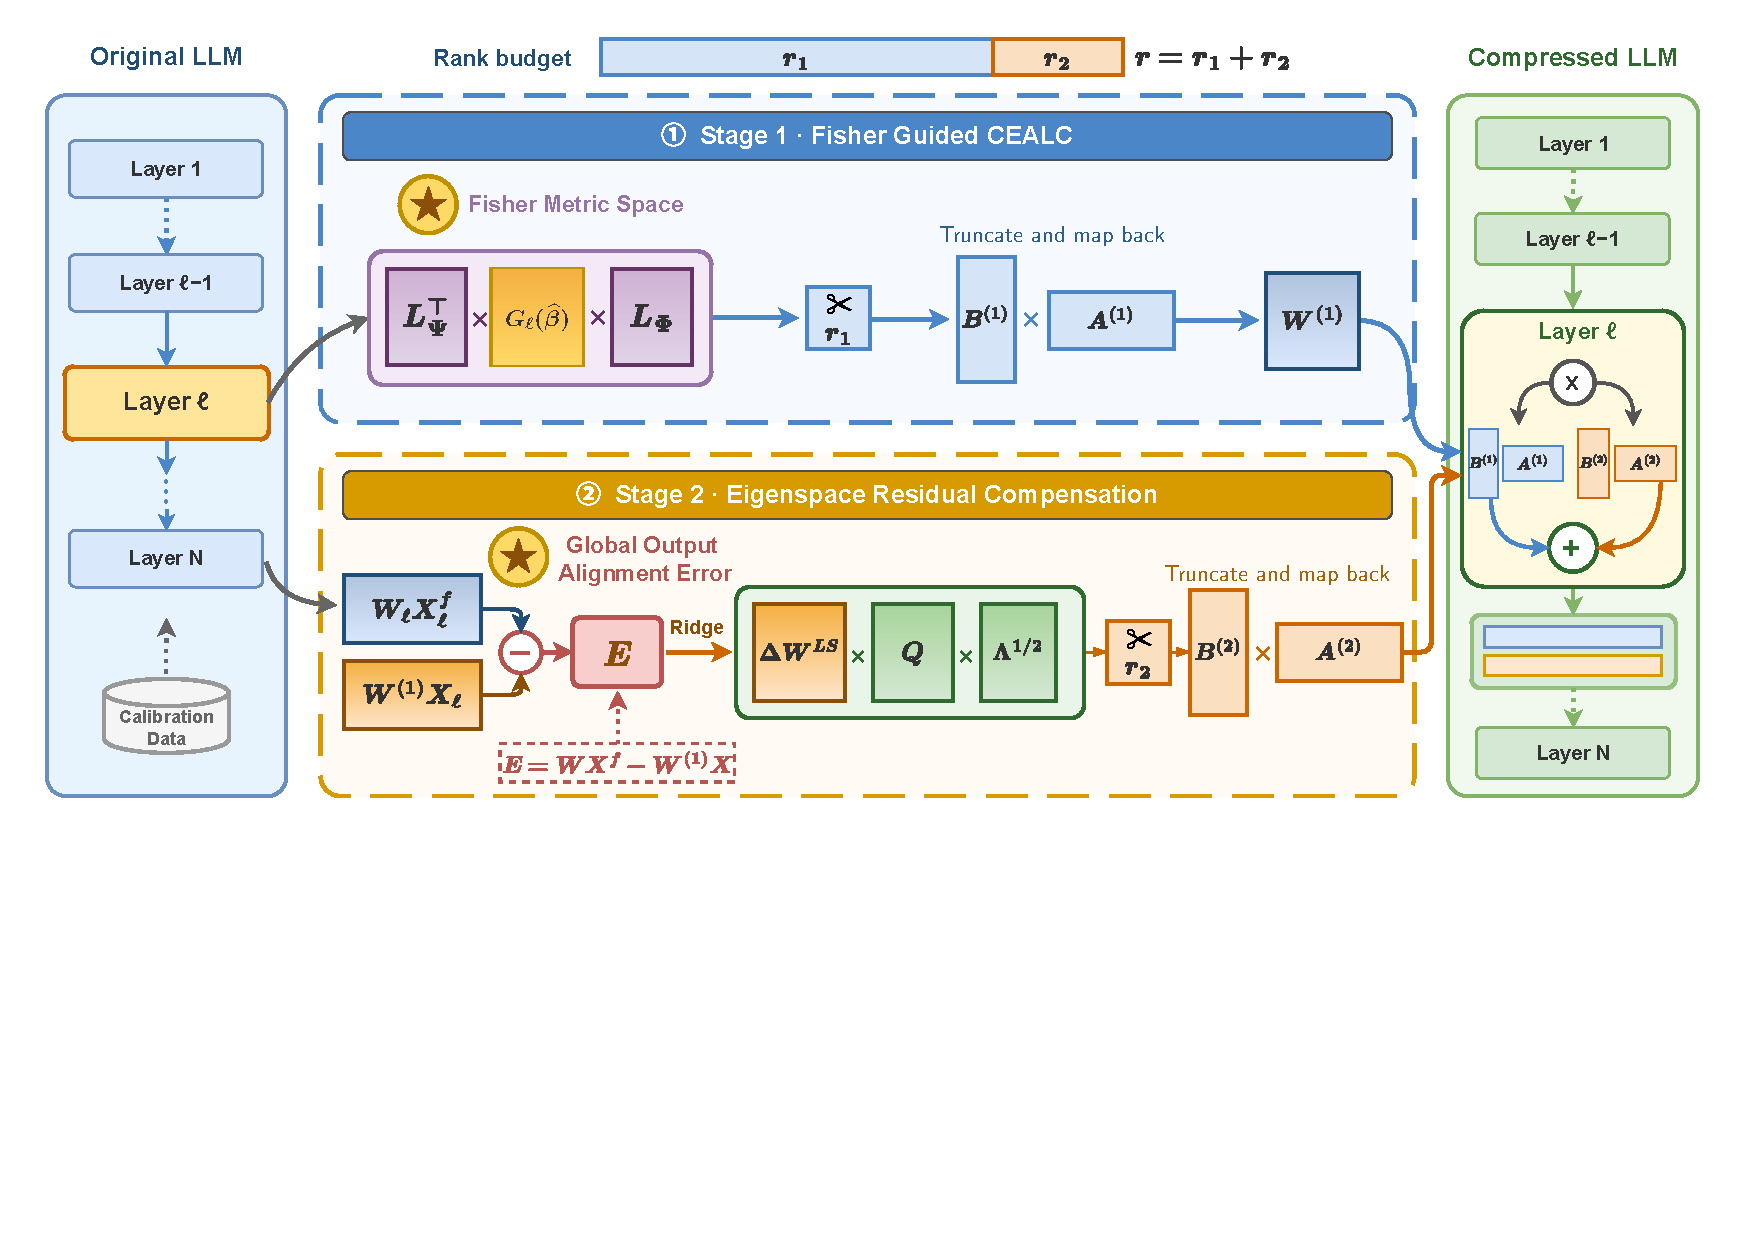
\includegraphics[width=\textwidth]{figs/Over_view_of_FR-SVD.pdf}
\caption{Overview of the FR-SVD framework for a single layer $\ell$. Calibration data is propagated through both the full-precision path (producing reference activations $X_\ell^f$) and the compressed path (producing compressed activations $X_\ell$), yielding the activation statistics $H_\ell$ and $\Delta_\ell$. Calibration loss gradients of the current model are used to jointly fit the Kronecker factors $\Phi_\ell$ and $\Psi_\ell$. \textbf{Stage~1} (Fisher-Guided CEALC) constructs the Fisher-space target matrix $G_\ell^F(\beta)$, selects $\widehat\beta$ using an energy-concentration heuristic, and performs rank-$r_1$ truncated SVD to produce the main compressed weight $W_\ell^{(1)}=B^{(1)}A^{(1)}$. \textbf{Stage~2} (Eigenspace Residual Compensation) computes the global alignment error $E_\ell$, solves the ridge regression in closed form, and projects the result to rank $r_2$ in the activation eigenspace to obtain $W_\ell^{\mathrm{comp}}=B^{(2)}A^{(2)}$. The total rank budget $r=r_1+r_2$ is shared between the two stages. At deployment, each compressed layer is retained as two parallel low-rank branches without reconstructing a dense matrix.}
\label{fig:overview}
\end{figure*}
